\chapter[Inverse Laplace Transforms]{Inverse Laplace Transforms:\\ Frobenius Traces, P\'olya Kernels\\ and Zeros}\label{ch:lap}

Langlands proposed that two different kinds of mathematics describe the same objects. On the Galois side an $L$ function is an Euler product built from Frobenius traces, one prime at a time, and it lives on the half plane $\operatorname{Re}s>1$ where the product converges. On the automorphic side the same $L$ function is a Mellin transform of a modular form read along the imaginary axis, it continues to the whole plane, it has a functional equation, and its nontrivial zeros lie in the critical strip, on the critical line if GRH holds. Reciprocity is the statement that these two descriptions agree.

Part~IV has used Laplace transforms mostly in the forward direction: the logarithm of an Euler product is the Laplace exponent of a L\'evy measure carried by the logarithms of prime powers (Chapter~\ref{ch:09}); a completed $L$ function is the two sided Laplace transform of a P\'olya kernel (Chapter~\ref{ch:10}, Lemma~\ref{lem:10bkernel}); the $2\sin^2$ lemma turns the L\'evy measure into a Thorin density (Lemma~\ref{lem:10dsin2}); and the heat trace is the Laplace transform of the counting measure of the squared ordinates of the zeros (Chapter~\ref{ch:10d}), which Chapter~\ref{ch:recip} computes from Frobenius traces (Definition~\ref{def:recipheat}). Some inversions have already appeared: Stieltjes inversion gives the closed form of the sine squared lemma (Chapter~\ref{ch:10d}) and the signed Thorin densities of Chapter~\ref{ch:scholze}, Mellin inversion proves Hecke's criterion (Proposition~\ref{prop:recipsym}), Fourier inversion computes the van Dantzig partner of $\Delta$ (Figure~\ref{fig:10dvdp}), and the zeros are recovered from the primes (Figure~\ref{fig:10dprimes}). This chapter collects the inverse transforms and uses them to pass between the faces of one $L$ function. The passage from the Galois side to the automorphic side still needs the analytic continuation that reciprocity supplies: it assumes that $\Lambda(s,\rho)$ is entire and bounded in vertical strips, which is Artin's conjecture for $\rho$; for the running example, the two dimensional representation $\rho_{23}$ of the Galois group of $x^3-x-1$, this is Hecke's theorem (Example~\ref{ex:ch3cubic}).

We organise an $L$ function, say $L(s,\rho)$, into four faces (Figure~\ref{fig:lapfaces}): the \emph{Galois face}, the measure $\nu_\alpha=\sum_n\Lambda_\rho(n)n^{-\alpha}\delta_{\log n}$, which is $x$ times the L\'evy measure of $\log L$ at $\alpha$, as in Lemma~\ref{lem:10dsin2}, and whose atoms carry the Frobenius traces; the \emph{transport face}, the $2\sin^2$ transform $U_\alpha$ of $\nu_\alpha$, which is the Thorin density of Lemma~\ref{lem:10dsin2} when $\nu_\alpha\ge0$; the \emph{automorphic face}, the P\'olya kernel $\Phi_\rho$, which is a modular form on the imaginary axis when $\rho$ is modular; and the \emph{zero face}, the family of Thorin densities $V_a$ of the completed function, which under GRH concentrates on the squared ordinates of the zeros as $a\downarrow0$ (Theorem~\ref{thm:10dshift}(iv)). For this face Figure~\ref{fig:lapfaces} shows the zeros themselves, as sign changes, and Figure~\ref{fig:lapzeta} shows the densities $V_a$ for $\zeta$. Schematically, with the Frobenius data at the top left, the transport below it, the zeros at the bottom centre and the kernel at the bottom right,
\[
\begin{array}{ccccc}
\Lambda_\rho(n) & \xrightarrow{\ \scriptstyle\mathrm{Laplace}\ } & \log L(\alpha+s,\rho) & \xrightarrow{\ \scriptstyle\mathrm{continue}\ } & \Lambda(\tfrac12+it,\rho)\\[2pt]
{\scriptstyle 2\sin^2}\big\downarrow\big\uparrow{\scriptstyle\mathrm{Bohr}} & & & & \big\downarrow{\scriptstyle\mathrm{Bromwich}}\\[2pt]
U_\alpha & \xrightarrow{\ \scriptstyle\mathrm{Cauchy}\ } & V_a & & \Phi_\rho(u)
\end{array}
\]
The bottom arrow completes the $L$ function, which adds explicit terms to $U_\alpha$ and gives $V_a$ at $a=\alpha-\frac12$, and then moves the basepoint, which adds or removes Cauchy noise. The inversions are classical (Section~\ref{sec:laptools}), and of the results below only the explicit error in (1), the readings of the Hecke GGC and of the Sato Tate law in (5), and the computations are new, as far as we know; (3) restates, through folded Cauchy variables and for every self dual $\pi$, what \cite{polson2017} proves for $\xi$ (see the Notes).
\begin{enumerate}
\item[(1)] The $2\sin^2$ transport is injective, and Bohr's mean value formula inverts it, with an explicit error for a Gaussian window (Theorem~\ref{thm:lapbohr}). Frobenius traces, times $-\frac12p^{-m\alpha}\log p$, are the Bohr coefficients of the transported density, and from the transported density of the weight one form $\eta(z)\eta(23z)$ we recover $\Lambda_\rho(n)$, $\rho=\rho_{23}$, for every $n\le64$ to $8.6\cdot10^{-9}$, and with it the Frobenius class at every unramified prime $p\le61$.
\item[(2)] For an odd two dimensional $\rho$ with $\Lambda(s,\rho)$ entire and bounded in vertical strips, Bromwich inversion on the critical line gives a kernel $\Phi_\rho$ with $\int\Phi_\rho(u)e^{tu}\,du=\Lambda(\frac12+t,\rho)$, and if $\rho$ comes from a weight one form $f$ of level $N$, then $\Phi_\rho(u)=2f(ie^u/\sqrt N)e^{u/2}$: this is Hecke's correspondence read backwards (Proposition~\ref{prop:lappolya}). For $\rho_{23}$ both hold by Hecke's theorem, with $f=\eta(z)\eta(23z)$. From $\Lambda(\frac12+it,\rho_{23})$, computed as $\zeta_K/\zeta$ through its continuation, $K$ the cubic field of $x^3-x-1$, the inversion gives a kernel that agrees with $2f(ie^u/\sqrt{23})e^{u/2}$ on $|u|\le3$ to $2.7\cdot10^{-16}$ in absolute value, the level of rounding.
\item[(3)] Moving the basepoint is a Cauchy semigroup (Theorem~\ref{thm:lapcauchy}), as in the proof of Theorem~\ref{thm:10dshift}: in the variable $r$, the square root of the Thorin variable, the Thorin measure at basepoint $\frac12+a$ is half the sum, over the zeros $\frac12+\beta+i\gamma$ of the completed function, of the laws of $|\gamma+(a-\beta)C|$ with $C$ standard Cauchy, and under GRH all the scales equal $a$. We check this against $1000$ zeros of $\zeta$ to $10^{-7}$.
\item[(4)] Inverting the Thorin law gives the universal tail found by Roynette and Yor \cite{roynetteyor2005} (Theorem~\ref{thm:laptail}). If $L$ has nonnegative coefficients $\Lambda_L(n)$, then for every $\alpha>1$ the Thorin variable $H$ of Lemma~\ref{lem:10dsin2} has mean $\frac12(\log L)''(\alpha)$, infinite variance, and a Pareto tail of index $\frac32$, $\Prob(H>t)\sim-(\log L)'''(\alpha)\,t^{-3/2}/(12\sqrt\pi)$.
\item[(5)] Two classical papers fit the same picture (Section~\ref{sec:lapspline}). Inverting the Laplace transform of a GGC with finitely many Thorin atoms gives a Gamma variable times a Curry Schoenberg B spline variable, the atomic case of a factorisation of James, Roynette and Yor \cite{jamesroynetteyor2008} (Theorem~\ref{thm:lapspline}); so the Hecke GGC of Definition~\ref{def:flthecke} is a Gamma variable times a B spline variable with knots $1/(\ell+1-a_\ell(f))$, and its density is proportional to $t^{g-1}$ times the Laplace transform of a B spline whose knots are the numbers $\ell+1-a_\ell(f)$, point counts when $f$ is rational. Among densities whose square root vanishes on the walls of the alcove, the Good and Gaskins roughness penalty is minimised exactly by the Sato Tate law, by an inequality of Huber for $\SU(2)$ and the Rayleigh principle for the alcove in general \cite{huber1974,berard1980}; the penalty is diagonal in the basis of irreducible characters, symmetric powers for $\SU(2)$, with weights the Laplace eigenvalues $|\lambda+\rho_G|^2$ (Theorem~\ref{thm:lapgg}).
\end{enumerate}
Section~\ref{sec:laptools} collects the classical inversion theorems in the form we use, with Feller's probabilistic proof of the Post Widder formula.

\section{Inverse Laplace transforms for probabilists}\label{sec:laptools}

Four inversion theorems do all the work. Lerch's theorem\index{Lerch's theorem} says that the forward transform loses nothing; Bromwich's formula\index{Bromwich inversion} inverts it along a vertical line; the Post Widder formula\index{Post Widder formula} inverts it on the real axis; and Stieltjes inversion\index{Stieltjes inversion} reads a Thorin measure off its boundary values.

\begin{theorem}[Lerch; uniqueness]\label{thm:laplerch}
If two positive or signed measures on $[0,\infty)$ have Laplace transforms that converge absolutely for $s>c$ and agree on a set with an accumulation point $s_0>c$, or on an arithmetic progression $c+kh$, $k\ge1$, with $h>0$, then the measures are equal. In particular two Dirichlet series $\sum a_nn^{-s}$ and $\sum b_nn^{-s}$ that converge absolutely and agree on such a set have $a_n=b_n$ for all $n$.
\end{theorem}

The second statement is the first applied to the measures $\sum a_n\delta_{\log n}$ and $\sum b_n\delta_{\log n}$, since $\sum a_nn^{-s}$ is their Laplace transform (\cite{widder1941}, Chapter~II, Theorems~6.2 and 6.3). For the Langlands programme it means that an identity $L(s,\rho)=L(s,\pi)$ on any interval of the half plane of absolute convergence is an identity of every Euler factor.

\begin{theorem}[Bromwich]\label{thm:lapbromwich}
Let $F(s)=\int_{\R}\Phi(u)e^{su}\,du$ converge absolutely on a vertical strip containing the line $\operatorname{Re}s=c$, and suppose $t\mapsto F(c+it)$ is integrable. Then $\Phi(u)=\frac1{2\pi}\int_{\R}F(c+it)e^{-(c+it)u}\,dt$ at every point of continuity of $\Phi$.
\end{theorem}

This is Fourier inversion applied to $\Phi(u)e^{cu}$ (\cite{widder1941}, Chapter~VI, Theorem~5a). For a Dirichlet series the transform is not integrable on vertical lines, and the same inversion, taken as a symmetric principal value, is Perron's formula, to which we return in Section~\ref{sec:lapperron}.

\begin{theorem}[Post Widder as a law of large numbers]\label{thm:lappostwidder}
Let $g$ be bounded and let $F(s)=\int_0^\infty e^{-sx}g(x)\,dx$ be its Laplace transform. For $k\ge1$ and $t>0$ let $Y_{k+1}$ be a Gamma variable with shape $k+1$ and scale $1$. Then
\[
\frac{(-1)^k}{k!}\Bigl(\frac kt\Bigr)^{k+1}F^{(k)}\Bigl(\frac kt\Bigr)=\E\,g\Bigl(\frac{t\,Y_{k+1}}k\Bigr)\ \longrightarrow\ g(t)
\]
as $k\to\infty$ at every point $t$ where $g$ is continuous.
\end{theorem}

\begin{proof}
Differentiating under the integral, $(-1)^kF^{(k)}(s)=\int_0^\infty x^ke^{-sx}g(x)\,dx$. With $s=k/t$ the function $x\mapsto(k/t)^{k+1}x^ke^{-kx/t}/k!$ is the density of $tY_{k+1}/k$, which gives the identity. By the weak law of large numbers $Y_{k+1}/k\to1$ in probability, so $tY_{k+1}/k\to t$, and since $g$ is bounded and continuous at $t$, $\E g(tY_{k+1}/k)\to g(t)$.
\end{proof}

Post found the formula and Widder extended it (\cite{widder1941}, Chapter~VII, Section~1); the reading as a law of large numbers is Feller's \cite{feller1971}. It shows what the inversion costs: the error is the Gamma smoothing of $g$ at relative width $k^{-1/2}$, so Post Widder converges like $1/k$ at smooth points, and in practice one uses contour methods \cite{talbot1979,abatewhitt2006}. Our computations use Talbot's contour.

\begin{theorem}[Stieltjes inversion of Thorin measures; \cite{stieltjes1894,akhiezer1965}]\label{thm:lapstieltjes}
Let $\varphi$ be the Laplace transform of a GGC with drift $a$ and Thorin measure $\tau$. On any open interval of $(0,\infty)$ where $\tau$ has a continuous density,
\[
\tau(z)=\frac1\pi\lim_{\varepsilon\downarrow0}\operatorname{Im}\frac{\varphi'}{\varphi}(-z+i\varepsilon).
\]
\end{theorem}

\begin{proof}
By the discussion after Definition~\ref{def:10bstieltjes}, $-\varphi'/\varphi(s)=a+\int\tau(dt)/(s+t)$, holomorphic off $(-\infty,0]$ by Lemma~\ref{lem:ch10nonvanish}. For $s=-z+i\varepsilon$, $\operatorname{Im}(t-z+i\varepsilon)^{-1}=-\varepsilon/((t-z)^2+\varepsilon^2)$, and $\frac1\pi\varepsilon/((t-z)^2+\varepsilon^2)$ is an approximate identity, so $\operatorname{Im}(-\varphi'/\varphi)(-z+i\varepsilon)\to-\pi\tau(z)$.
\end{proof}

As noted after Lemma~\ref{lem:10dsin2}, the theorem applied to $\varphi(s)=e^{b\sqrt s}f(\alpha)/f(\alpha+\sqrt s)$, with $\sqrt s=i\sqrt z$ on the upper side of the cut, gives the closed form \eqref{eq:10dU}. For $\varphi=1/G_\pi$ the right side before the limit is the signed density $u_\varepsilon$ of Chapter~\ref{ch:scholze}.

\section{Inverting the sine squared transport}\label{sec:lapbohr}

Lemma~\ref{lem:10dsin2} goes from the Galois face to the transport face. Its arithmetic content is in the closed form: for an $L$ function with $-L'/L(s)=\sum_n\Lambda_L(n)n^{-s}$ and for $\alpha>1$, by \eqref{eq:10dU},
\begin{equation}\label{eq:lapg}
g_\alpha(r):=2\pi r\,U_\alpha(r^2)=\operatorname{Re}\frac{L'}L(\alpha+ir)-\frac{L'}L(\alpha)=\sum_{n\ge2}\frac{\Lambda_L(n)}{n^\alpha}\bigl(1-\cos(r\log n)\bigr),
\end{equation}
which makes sense whether or not $\Lambda_L(n)\ge0$ (the middle expression assumes the $\Lambda_L(n)$ real, as for a self dual $L$; in general it reads $\frac12\bigl(\frac{L'}L(\alpha+ir)+\frac{L'}L(\alpha-ir)\bigr)-\frac{L'}L(\alpha)$); $U_\alpha$ is the density $U_{\mathrm{ar}}$ of Section~\ref{sec:10daway}, and $g_\alpha$ is unrelated to the function of that name in the van Dantzig pairs of Chapter~\ref{ch:10d}. When $\Lambda_L\ge0$, $U_\alpha$ is a Thorin density; when $\Lambda_L$ is signed, as for $\eta(z)\eta(23z)$, it is a signed density, the transport of a signed L\'evy measure. A mean value inverts it.

\begin{theorem}[inverse of the sine squared transport; after Bohr \cite{besicovitch1932}]\label{thm:lapbohr}
Let $\nu=\sum_jc_j\delta_{x_j}$ with distinct $x_j>0$ and $\sum_j|c_j|<\infty$, and let $g(r)=\int(1-\cos rx)\,\nu(dx)$. For $R>0$ write $\mathcal G_R[h]=\int_0^\infty h(r)e^{-r^2/(2R^2)}dr\big/\int_0^\infty e^{-r^2/(2R^2)}dr$. Then
\[
\mathcal G_R\bigl[g(r)\cos(rx_k)\bigr]=\sum_jc_j\Bigl[e^{-x_k^2R^2/2}-\tfrac12e^{-(x_j-x_k)^2R^2/2}-\tfrac12e^{-(x_j+x_k)^2R^2/2}\Bigr],
\]
so that, with $\delta_k=\min(x_k,\inf_{j\ne k}|x_j-x_k|)$, assumed positive,
\[
\Bigl|c_k+2\mathcal G_R\bigl[g(r)\cos(rx_k)\bigr]\Bigr|\le2\Bigl(\sum_j|c_j|\Bigr)e^{-\delta_k^2R^2/2}.
\]
In particular $c_k=-2\lim_{R\to\infty}\mathcal G_R[g(r)\cos(rx_k)]$, the same limit holds for the plain Bohr mean $\lim\frac1R\int_0^R$, and the transport $\nu\mapsto g$ is injective.
\end{theorem}

\begin{proof}
The Gaussian characteristic function gives $\mathcal G_R[\cos(ar)]=e^{-a^2R^2/2}$ for real $a$. Expand
\[
g(r)\cos(rx_k)=\sum_jc_j\Bigl[\cos(rx_k)-\tfrac12\cos\bigl(r(x_j-x_k)\bigr)-\tfrac12\cos\bigl(r(x_j+x_k)\bigr)\Bigr];
\]
the series converges uniformly, so $\mathcal G_R$ may be applied term by term, which gives the identity. The term $j=k$ contributes $c_k[e^{-x_k^2R^2/2}-\frac12-\frac12e^{-2x_k^2R^2}]$, so $c_k+2\mathcal G_R[\cdot]$ is the sum of
\[
c_k\bigl(2e^{-x_k^2R^2/2}-e^{-2x_k^2R^2}\bigr),
\]
of size at most $2|c_k|e^{-\delta_k^2R^2/2}$, and of the terms $c_j(2e_0-e_j^{-}-e_j^{+})$ for $j\ne k$. Here $e_0=e^{-x_k^2R^2/2}$ and $e_j^\pm=e^{-(x_j\pm x_k)^2R^2/2}$ lie in $[0,e^{-\delta_k^2R^2/2}]$ because $x_k$ and $|x_j\pm x_k|$ are at least $\delta_k$, so each such term has size at most $2|c_j|e^{-\delta_k^2R^2/2}$. For the plain mean, $\frac1R\int_0^R\cos(ar)\,dr\to\delta_{a,0}$ and uniform convergence gives the same limit. If $g=0$ every $c_k$ vanishes, which is injectivity.
\end{proof}

The limit is Bohr's formula for the Fourier coefficients of an almost periodic function\index{Bohr mean}, and injectivity is his uniqueness theorem (\cite{besicovitch1932}, Chapter~I, Sections~3 and 4; for Dirichlet series, Chapter~III, Section~3); the Gaussian window makes the error explicit.

\begin{corollary}[Frobenius traces from the transported density]\label{cor:lapfrob}
Let $L(s)=\sum a_nn^{-s}$ have an Euler product with $-L'/L(s)=\sum\Lambda_L(n)n^{-s}$ absolutely convergent for $\operatorname{Re}s>1$, as for Artin $L$ functions and, by the Rankin Selberg method of Jacquet and Shalika \cite{jacquetshalika1981} and the Cauchy Schwarz inequality, for cuspidal automorphic ones. For $\alpha>1$ and $n\ge2$,
\[
\Lambda_L(n)=-2n^\alpha\lim_{R\to\infty}\mathcal G_R\bigl[g_\alpha(r)\cos(r\log n)\bigr],
\]
and the error at a finite $R$ is at most
\[
2n^\alpha\Bigl(\sum_m|\Lambda_L(m)|m^{-\alpha}\Bigr)e^{-\delta_n^2R^2/2},\qquad\delta_n=\log(1+1/n).
\]
If $L=L(s,\rho)$ for an Artin representation unramified at $p$, then $\Lambda_L=\Lambda_\rho$ and $\tr\rho(\Frob_p^m)=\Lambda_\rho(p^m)/\log p$, so by Theorem~\ref{thm:lapfaces} the transported density on any interval of $r$ determines every Frobenius trace.
\end{corollary}

\begin{proof}
Apply Theorem~\ref{thm:lapbohr} to $\nu_\alpha=\sum\Lambda_L(n)n^{-\alpha}\delta_{\log n}$, with $x_n=\log n$, of weight $0$ when $n$ is not a prime power; every other atom lies at distance at least $\log(1+1/n)$ from $\log n$, and $\log(1+1/n)<\log n$.
\end{proof}

\begin{theorem}[reciprocity on any face]\label{thm:lapfaces}
Let $L_1,L_2$ be Euler products as in Corollary~\ref{cor:lapfrob}, for instance $L^S(s,\rho)$ and $L^S(s,\pi)$ with the Euler factors at a finite set $S$ removed. Fix $\alpha>1$. The following are equivalent.
\begin{enumerate}
\item[(i)] $L_1(s)=L_2(s)$ for $s$ in some interval of $(1,\infty)$.
\item[(ii)] The Galois faces agree: $\Lambda_{L_1}(n)=\Lambda_{L_2}(n)$ for all $n$, that is $\nu^{(1)}_\alpha=\nu^{(2)}_\alpha$.
\item[(iii)] The transport faces agree: $g^{(1)}_\alpha=g^{(2)}_\alpha$ on some interval $[0,r_0)$.
\end{enumerate}
\end{theorem}

\begin{proof}
(i) implies (ii) by Theorem~\ref{thm:laplerch} applied to $\log L_j=\sum\Lambda_{L_j}(n)n^{-s}/\log n$, and (ii) implies (iii) by \eqref{eq:lapg}. If (iii) holds, both $g^{(j)}_\alpha$ extend holomorphically to the strip $|\operatorname{Im}r|<\alpha-1$, since $\sum|\Lambda_{L_j}(n)|n^{-\alpha}\cosh(y\log n)<\infty$ for $|y|<\alpha-1$; they agree on an interval, hence on all of $\R$, and Theorem~\ref{thm:lapbohr} gives (ii). Finally (ii) gives $\log L_1=\log L_2$ on $\operatorname{Re}s>1$.
\end{proof}

So a reciprocity law may be tested on either face, and a failure shows up on both. Figure~\ref{fig:lapfaces} shows this for the running example of the book (Example~\ref{ex:ch3cubic}). The $q$ expansion of $\eta(z)\eta(23z)$ was computed from Euler's pentagonal series, and the Frobenius data of $x^3-x-1$ from the splitting of primes in its cubic field. They agree at all $17984$ primes and all $18120$ prime powers below $2\cdot10^5$, including $a_{23}=1$. So the two transported densities at $\alpha=1.5$ coincide exactly, while a single wrong coefficient, $a_{59}$ changed from $2$ to $0$, is visible at every $r$ except the points $r=2\pi k/\log59$.

The inverse arrow is the substantial one. We summed $L(s)$ and $L'(s)$ for the modular form from its first $30000$ coefficients at $s=2+ir$, $0\le r\le2700$, formed $g_2(r)$ from \eqref{eq:lapg}, and applied Corollary~\ref{cor:lapfrob} with $R=450$. The recovered $\Lambda_\rho(n)$ agree with the Frobenius values for every $n\le64$ to $8.6\cdot10^{-9}$; the error comes from the truncation of the window at $r=6R$, not from the theorem. Dividing by $\log p$ returns the Frobenius labels: $-1$ at $p=2,3,13,29,31,41,47$, where $x^3-x-1$ has no root, $0$ at $p=5,7,11,17,19,37,43,53,61$, the primes inert in $\Q(\sqrt{-23})$, $2$ at $p=59$, the first prime that splits completely, and $1$ at the ramified prime $23$. For $n=59$ the bound of Corollary~\ref{cor:lapfrob} is $1.1\cdot10^{-9}$, below the observed error $2.9\cdot10^{-9}$, and the observed errors exceed the bound at every $n\le60$; but the bound allows for atoms at $n\pm1$, while the nearest prime powers to $59$ are $53$ and $61$, so the exact Gaussian mean is far more accurate than the bound, and the observed errors come from the window. With exact atoms and the same truncated window the error is again $8.6\cdot10^{-9}$, largest at $n=60$; with the window cut at $r=8R$ it falls to $1.7\cdot10^{-11}$. In this sense the transported density of the modular form \emph{contains} the Galois representation, and Corollary~\ref{cor:lapfrob} reads it off.

\begin{figure}[!htbp]
\centering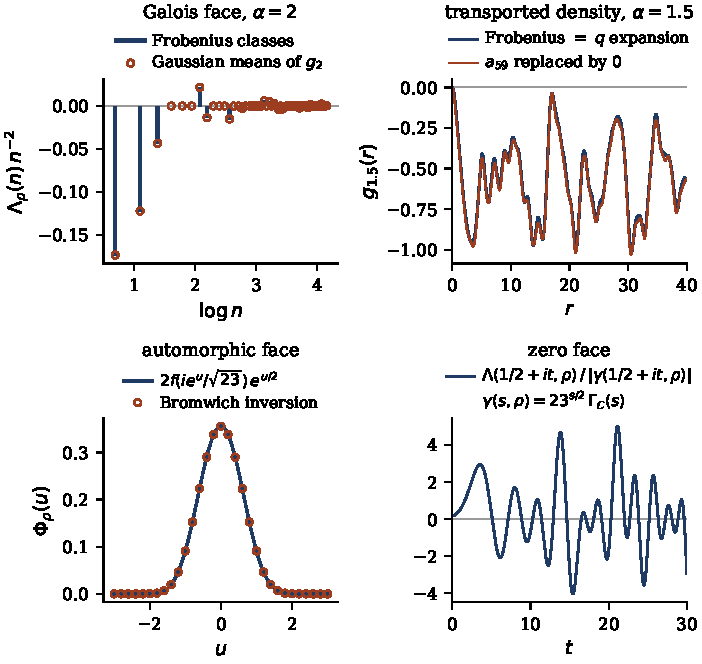
\includegraphics[width=\textwidth]{figs/lap_faces.pdf}
\caption{Four faces of $L(s,\rho)=L(s,\eta(z)\eta(23z))$, $\rho$ the two dimensional representation of the Galois group of the splitting field of $x^3-x-1$. Top left: the Galois face at $\alpha=2$, the atoms $\Lambda_\rho(n)n^{-2}$, $n\le64$, from Frobenius classes (bars) and as Gaussian means of the transported density $g_2$ computed from the modular form (circles), Corollary~\ref{cor:lapfrob}. Top right: the transport face, the transported density $g_{1.5}$ from Frobenius and from the $q$ expansion (one curve, the two being identical), and with $a_{59}$ replaced by $0$. Bottom left: the automorphic face, the kernel $\Phi_\rho$ computed by Bromwich inversion of $\Lambda(\frac12+it,\rho)$ (circles) against $2f(ie^u/\sqrt{23})e^{u/2}$ for $f=\eta(z)\eta(23z)$ (line), Proposition~\ref{prop:lappolya}. Bottom right: for the zero face, the zeros themselves, as the sign changes of the real function $\Lambda(\frac12+it,\rho)/|\gamma(\frac12+it,\rho)|$, with $\gamma(s,\rho)=23^{s/2}\Gamma_\C(s)$ the gamma factor of Section~\ref{sec:10bcompletion}, of absolute value $|L(\frac12+it,\rho)|$.}\label{fig:lapfaces}
\end{figure}

\section{Bromwich inversion: from the Artin \texorpdfstring{$L$}{L} function to the modular form}\label{sec:lappolya}

The automorphic face of a degree two $L$ function is a function on the imaginary axis, and the Mellin transform makes it a two sided Laplace transform, as in Section~\ref{sec:02mellin} and \eqref{eq:recipmellin}. Write $\Gamma_\C(s)=2(2\pi)^{-s}\Gamma(s)=\Gamma_\R(s)\Gamma_\R(s+1)$.

\begin{proposition}[Mellin inversion of an Artin $L$ function; after Hecke \cite{hecke1936}]\label{prop:lappolya}
Let $\rho$ be an odd two dimensional Artin representation of conductor $N$, and assume that its completed $L$ function $\Lambda(s,\rho)=N^{s/2}\Gamma_\C(s)L(s,\rho)$ is entire and bounded in vertical strips (Artin's conjecture for $\rho$). Put
\[
\Phi_\rho(u)=\frac1{2\pi}\int_{\R}\Lambda(\tfrac12+it,\rho)e^{-itu}\,dt .
\]
Then $\Lambda(\frac12+t,\rho)=\int_{\R}\Phi_\rho(u)e^{tu}\,du$ for real $t$. If $\rho$ is attached to a weight one newform $f$, then $\Phi_\rho(u)=2f(ie^u/\sqrt N)e^{u/2}$. If moreover $\Lambda(s,\rho)=\Lambda(1-s,\rho)$, then $\Phi_\rho$ is even, and if $f$ is positive on the imaginary axis then $\Phi_\rho/\Lambda(\frac12,\rho)$ is the density of a symmetric random variable.
\end{proposition}

\begin{proof}
By the functional equation $\Lambda(s,\rho)=W(\rho)\Lambda(1-s,\bar\rho)$ and the Phragm\'en Lindel\"of principle, boundedness in vertical strips gives polynomial growth of $L(\sigma+it,\rho)$ in $|t|$, uniformly for $\sigma$ in compact sets, and Stirling's formula then gives exponential decay of $\Lambda(\sigma+it,\rho)$ in $|t|$. As in the proof of Lemma~\ref{lem:10bkernel}, $\frac1{2\pi}\int_{\R}\Lambda(\frac12+x+it,\rho)e^{-(x+it)u}\,dt$ does not depend on $x$, so it equals $\Phi_\rho(u)$, it decays faster than any exponential as $u\to\pm\infty$, and $\int_{\R}\Phi_\rho(u)e^{zu}\,du=\Lambda(\frac12+z,\rho)$ for every complex $z$, which at real $z=t$ is the first statement. If $\rho$ corresponds to $f$, then $\Lambda(s,\rho)$ is twice the function $\Lambda(s)$ of Section~\ref{sec:recipfaces} with $k=1$, because $\Gamma_\C(s)=2(2\pi)^{-s}\Gamma(s)$. Both sides of the second identity in \eqref{eq:recipmellin} are entire in $t$, because $f(iy)$ decays exponentially as $y\to\infty$ and, by the Fricke involution, as $y\to0$, so that identity and the uniqueness of the Fourier transform give $\Phi_\rho=2\Phi_f$, with $\Phi_f(u)=f(ie^u/\sqrt N)e^{u/2}$ the P\'olya kernel of Chapter~\ref{ch:recip}. The last statements are Hecke's criterion (Proposition~\ref{prop:recipsym}) and positivity.
\end{proof}

The input to the integral is Galois data together with analytic continuation. An Artin $L$ function is determined by the Frobenius classes, and its meromorphic continuation and functional equation follow from Brauer's induction theorem \cite{brauer1947}; that $\Lambda(s,\rho_{23})$ is entire and bounded in strips is Hecke's theorem, since $L(s,\rho_{23})=\zeta_K(s)/\zeta(s)$, $K=\Q[x]/(x^3-x-1)$, is the $L$ function of the weight one form $\eta(z)\eta(23z)$ (Example~\ref{ex:ch3cubic}). PARI computes $\Lambda(s,\rho_{23})$ as this quotient, using the functional equations of $\zeta_K$ and $\zeta$. The output is a function on the imaginary axis, and reciprocity says that it is a modular form. We evaluated $\Lambda(\frac12+it,\rho)$ for $0\le t\le60$ in steps of $0.005$ (it is real there, and below $10^{-26}$ in absolute value beyond $t=40$), integrated, and compared $\Phi_\rho$ with $2f(ie^u/\sqrt{23})e^{u/2}$ for $f=\eta(z)\eta(23z)$, summed from $4000$ terms of its $q$ expansion. On $|u|\le3$ the two agree to $2.7\cdot10^{-16}$ in absolute value, the level of rounding (Figure~\ref{fig:lapfaces}, bottom left). The kernel is positive, with $\int\Phi_\rho=\Lambda(\frac12,\rho)=0.5390$, so $\Phi_\rho/\Lambda(\frac12,\rho)$, the P\'olya kernel\index{P\'olya kernel} $\Phi^{\mathrm{sd}}$ of Lemma~\ref{lem:10bkernel} for the weight one form, is the density of a symmetric random variable, its P\'olya variable (Chapter~\ref{ch:recip} uses $\Phi_f=\frac12\Phi_\rho$).

The proposition also says where the deep content of reciprocity sits. The inverse transform exists once $\Lambda(s,\rho)$ is entire and bounded in strips. That the result is modular, transforming correctly under all of $\Gamma_0(N)$ with its character and not merely under the Fricke involution, follows from Weil's converse theorem\index{converse theorem} (\cite{weil1967}, Satz~2) once the twists $\Lambda(s,\rho\otimes\chi)$ are also entire, bounded in strips and satisfy their functional equations; for two dimensional Artin representations this is Th\'eor\`eme~4.10 of Deligne and Serre \cite{deligneserre1974}. For odd irreducible $\rho$ these hypotheses are now known, by Hecke, Langlands and Tunnell \cite{langlands1980,tunnell1981} when the projective image is solvable and in general through Serre's conjecture, proved by Khare and Wintenberger \cite{kharewintenberger2009,kharewintenberger2009b} with work of Kisin \cite{kisin2009} (Chapter~\ref{ch:flt}).

\section{Moving the basepoint: the Cauchy semigroup}\label{sec:lapcauchy}

The Galois face lives at basepoints $\alpha>1$, the zeros at the centre. Theorem~\ref{thm:10dshift} gives a Thorin representation at every basepoint to the right of all zeros, and its proof writes the Thorin density as a sum of Poisson kernels over the zeros (see also Proposition~\ref{prop:10dsmooth} and Section~\ref{sec:sf:strip}); we now read that sum as a law. Let $\pi$ be self dual and let $\Xi^{\mathrm{sd}}_\pi(w)$ be $\Lambda(\frac12+w,\pi)$ divided by the power of $w$ that removes any zero at $w=0$, as in Definition~\ref{def:10bxi}; for $\zeta$ use $\Xi_\zeta(w)=\xi(\frac12+w)$ in its place below. Since $\Xi_\pi=(\Xi^{\mathrm{sd}}_\pi)^2$, Theorem~\ref{thm:10dshift} holds for $\Xi^{\mathrm{sd}}_\pi$ with every Thorin density halved, as in the last sentence of Theorem~\ref{thm:10bmain}, and below $V_a$ and $H_a$ denote this version. The function $\Xi^{\mathrm{sd}}_\pi$ is even and entire of order at most one (Lemma~\ref{lem:10bcompletion}(iii) and (v)); its zeros $z=\beta+i\gamma$, counted with multiplicity, form a multiset $\mathcal Z$ closed under $z\mapsto-z$ and $z\mapsto\bar z$, and $|\beta|<\frac12$. Let $C$ denote a standard Cauchy variable, with density $1/(\pi(1+x^2))$.

\begin{theorem}[zeros plus Cauchy noise; after \cite{polson2017,polson2018vdp}]\label{thm:lapcauchy}
Let $a>|\beta|$ for every $z=\beta+i\gamma$ in $\mathcal Z$; this holds unconditionally for $a\ge\frac12$. In the variable $r>0$, the square root of the Thorin variable, the Thorin measure of the GGC $H_a$ of Theorem~\ref{thm:10dshift}, $\Xi^{\mathrm{sd}}_\pi(a)/\Xi^{\mathrm{sd}}_\pi(a+\sqrt s)=\E e^{-sH_a}$, is
\[
V_a(r^2)\,2r\,dr=\frac12\sum_{z\in\mathcal Z}\operatorname{Law}\bigl(|\gamma+(a-\beta)C|\bigr)(dr),\qquad r>0 .
\]
Under GRH this is $\sum_{\gamma>0}\operatorname{Law}(|\gamma+aC|)$ for every $a>0$, a superposition of folded Cauchy laws centred at the ordinates with common scale $a$. For $b>0$, $V_{a+b}$ is obtained from $V_a$ by adding independent Cauchy noise of scale $b$ before folding, and on the Galois face, for $a>\frac12$, this is multiplication by $e^{-bx}$ of the whole L\'evy measure of $\log\Xi^{\mathrm{sd}}_\pi$ at basepoint $a$, archimedean and polynomial factors included.
\end{theorem}

\begin{proof}
By the definition of $V_a$ in Theorem~\ref{thm:10dshift}, $V_a(r^2)\,2r=\frac1\pi\operatorname{Re}(\log\Xi^{\mathrm{sd}}_\pi)'(a+ir)$, and by the Hadamard product $(\log\Xi^{\mathrm{sd}}_\pi)'(w)$ is the sum of $(w-z)^{-1}$ over $z\in\mathcal Z$, taken in pairs $\pm z$. For $z=\beta+i\gamma$,
\[
\frac1\pi\operatorname{Re}\frac1{a+ir-z}=\frac1\pi\frac{a-\beta}{(a-\beta)^2+(r-\gamma)^2},
\]
the density at $r$ of $\gamma+(a-\beta)C$, positive because $a>|\beta|$. The symmetries of $\mathcal Z$ make the sum even in $r$, so on $r>0$ it is half the sum of the folded densities, as stated. Under GRH, $\mathcal Z=\{\pm i\gamma\}$, $\beta=0$, and the two zeros $\pm i\gamma$ give the two halves of $\operatorname{Law}(|\gamma+aC|)$. Cauchy laws are stable, $(a-\beta)C+bC'$ having the law of $(a+b-\beta)C$ for independent $C,C'$, which is the semigroup. On the Galois face, for $a>\frac12$ the L\'evy measure of $\log\Xi^{\mathrm{sd}}_\pi$ at basepoint $a$ is $e^{-ax}\mu(dx)/x$ with $\mu$ independent of $a$, as in \eqref{eq:10dlk} with $\nu$ now signed, so moving to $a+b$ multiplies it by $e^{-bx}$; and $e^{-b|x|}$ is the Fourier transform of the Cauchy density of scale $b$.
\end{proof}

The Poisson kernel form of $V_a$ is in the proof of Theorem~\ref{thm:10dshift} and in Proposition~\ref{prop:10dsmooth}, for $\xi$ in \cite{polson2018vdp} (Theorem~18 and Remark~21), and Chapter~\ref{ch:squarefree} writes the density contributed by a pair of zeros off the line as a sum of two Poisson kernels (Section~\ref{sec:sf:strip}); the semigroup\index{Cauchy semigroup} in the basepoint is the backward Cauchy flow of \cite{polson2017} (Section~8 and Theorem~9.2). The theorem states these facts through folded Cauchy variables and for every self dual $\pi$; for $\xi$, its distribution function is the sum of arctangents of Theorem~8.2 of \cite{polson2017}. We check it below against $1000$ zeros of $\zeta$. Chapter~\ref{ch:scholze} smooths the atoms at the squared ordinates by Lorentzians of width $\varepsilon$, through Stieltjes inversion; here the smoothing is in the variable $r$, its scale is $a-\beta$, and it comes from moving the basepoint.

The theorem gives a probabilistic picture of the passage from the Galois face to the zeros. At $a\ge\frac12$, where the Thorin measure is positive unconditionally, each zero is seen through Cauchy noise of scale between $a-\frac12$ and $a+\frac12$. As $a$ decreases the noise shrinks, and GRH is the statement that it can be shrunk to zero for every zero at once; a zero with $\beta>0$ would make the scale $a-\beta$ negative for $a<\beta$, a negative Cauchy density. The proof of Theorem~\ref{thm:10dshift}(iv) and the remark after it use this sign change, and the criterion of Hinkkanen and Lagarias \cite{hinkkanen1997,lagarias1999}, that the Riemann hypothesis holds if and only if $\operatorname{Re}\xi'/\xi(s)>0$ for $\operatorname{Re}s>\frac12$, is the same statement about scales: its proof (\cite{lagarias1999}, Section~2) adds the same Poisson kernels term by term.

For $\zeta$ we compared $\frac1\pi\operatorname{Re}(\Xi_\zeta'/\Xi_\zeta)(a+ir)$ on $0<r\le50$, computed from $\zeta$, $\Gamma$ and the polynomial factor, with the Cauchy superposition over the first $1000$ zeros plus a smooth tail beyond $\gamma_{1000}=1419.42$. The maximal differences are $9.2\cdot10^{-8}$, $3.7\cdot10^{-8}$ and $9.2\cdot10^{-9}$ at $a=0.5$, $0.2$ and $0.05$, against peak values $0.72$, $1.63$ and $6.37$ (Figure~\ref{fig:lapzeta}, left).

\section{Inverting the Thorin law: a universal tail}\label{sec:laptail}

The Thorin variable $H$ of Lemma~\ref{lem:10dsin2} is the second member of a Wald couple of Roynette and Yor \cite{roynetteyor2005}, who found the tail of its density. Inverting the Laplace transform recovers their result, and the inversion has a universal feature.

\begin{theorem}[the tail of the Thorin variable; Roynette and Yor \cite{roynetteyor2005}]\label{thm:laptail}
Let $\Lambda_f(n)\ge0$, not all zero, and let $f(s)=\exp\bigl(\sum_{n\ge2}\Lambda_f(n)n^{-s}/\log n\bigr)$ converge absolutely for $\operatorname{Re}s>\alpha_0$. For $\alpha>\alpha_0$ let $H$ be the GGC of Lemma~\ref{lem:10dsin2} for $f$ at the basepoint $\alpha$, with $\nu_\alpha=\sum_n\Lambda_f(n)n^{-\alpha}\delta_{\log n}$, so that
\[
\E e^{-sH}=e^{b\sqrt s}\,\frac{f(\alpha)}{f(\alpha+\sqrt s)},\qquad b=\frac{f'}f(\alpha)<0 .
\]
Then
\[
\E H=\tfrac12(\log f)''(\alpha),\qquad \E H^2=\infty,
\]
and the density $p$ of $H$ satisfies
\[
p(t)\sim A\,t^{-5/2},\qquad \Prob(H>t)\sim\tfrac23A\,t^{-3/2},
\]
where
\[
A=\frac{-(\log f)'''(\alpha)}{8\sqrt\pi}=\frac1{8\sqrt\pi}\sum_n\frac{\Lambda_f(n)(\log n)^2}{n^\alpha}.
\]
\end{theorem}

This is Proposition~I.3.1 and Remarque~I.3.2 of \cite{roynetteyor2005} for $c(dx)=\nu_\alpha(dx)/x$, their $H$ being $2H$ here, with the density given by part~(1) of that proposition; for $\zeta$ the variable and its mean are their Th\'eor\`eme~V.1.1. They reach the constant through a Tauberian theorem; the proof below uses Doetsch's transfer theorem, which also gives the next terms.

\begin{proof}
Write $\varphi(s)=\E e^{-sH}$ and $w=\sqrt s$. Since $\log f$ is holomorphic near $\alpha$, Taylor's formula gives $\log f(\alpha+w)=\log f(\alpha)+bw+\frac12f_2w^2+\frac16f_3w^3+O(w^4)$ with $f_k=(\log f)^{(k)}(\alpha)$, so
\[
\log\varphi(s)=-\tfrac12f_2\,s-\tfrac16f_3\,s^{3/2}+O(s^2),
\]
uniformly as $s\to0$ in the slit plane. Differentiating the series of $\log f$ term by term gives $f_2=\sum\Lambda_f(n)\log n\,n^{-\alpha}$ and $f_3=-\sum\Lambda_f(n)(\log n)^2n^{-\alpha}<0$. The mean is the coefficient of $-s$. The term $s^{3/2}$ is not twice differentiable at $0$, so $\E H^2=\infty$. The function $\varphi$ is holomorphic on $\C\setminus(-\infty,0]$, because $\operatorname{Re}\sqrt s>0$ there and $f$ has no zeros on $\operatorname{Re}s>\alpha_0$, and $\varphi(s)\to0$ as $|s|\to\infty$, uniformly in every sector $|\arg s|\le\pi-\delta$, since $f(\alpha+\sqrt s)\to1$ and $b<0$. Since $\log f(\alpha+w)$ is analytic in $w$, the expansion of $\varphi$ at $0$ is a power series in $\sqrt s$, so after $s^{3/2}$ the next nonintegral power is $s^{5/2}$. Doetsch's transfer theorem for Laplace transforms with algebraic singularities \cite{doetsch1974}, whose hypotheses are these two properties, turns each term $cs^\lambda$, $\lambda\notin\{0,1,2,\dots\}$, of the expansion at $0$ into a term $ct^{-\lambda-1}/\Gamma(-\lambda)$ of the density at infinity. With $c=-f_3/6$, $\lambda=\frac32$ and $\Gamma(-\frac32)=\frac43\sqrt\pi$ this is $A$. Integrating gives the tail of the distribution function.
\end{proof}

The index $\frac32$ does not depend on $f$ or on $\alpha$. By Step~3 of the proof of Lemma~\ref{lem:10dsin2}, $H$ has the L\'evy density
\[
\frac{k(y)}y=\frac1{2\sqrt\pi\,y^{3/2}}\int_0^\infty\bigl(1-e^{-x^2/(4y)}\bigr)\,\nu_\alpha(dx)\sim Ay^{-5/2},\qquad y\to\infty,
\]
since $1-e^{-x^2/(4y)}\sim x^2/(4y)$: the L\'evy measure already has the tail of the theorem, the power coming from the stable law of index $\frac12$ in Step~1, and the theorem says that the law inherits it. What depends on the arithmetic is the constant, $(8\sqrt\pi)^{-1}$ times the second moment $\int x^2\nu_\alpha(dx)$ of the Galois face. Since $8\sqrt\pi A(\alpha)=\sum_n\Lambda_f(n)(\log n)^2n^{-\alpha}$ is a Dirichlet series, the function $\alpha\mapsto A(\alpha)$ on an interval determines $\Lambda_f$, by Theorem~\ref{thm:laplerch}.

The variable $H_a$ of Theorem~\ref{thm:lapcauchy}, for $\Xi=\Xi^{\mathrm{sd}}_\pi$ or $\Xi_\zeta$, is not compensated: its transform $\Xi(a)/\Xi(a+\sqrt s)$ contains the factor $e^{-b_a\sqrt s}$ of a positive stable law of index $\frac12$, with $b_a=(\Xi'/\Xi)(a)>0$. So $\Prob(H_a>t)\sim b_a/\sqrt{\pi t}$ for every $a$ to which Theorem~\ref{thm:10dshift}(i) applies (every $a\ge\frac12$, and every $a>0$ under GRH), while under GRH the limit at $a=0$, the explosion time of Theorem~\ref{thm:hitexplosion}, has an exponential tail. With that factor removed, $e^{b_a\sqrt s}\,\Xi(a)/\Xi(a+\sqrt s)$ is a GGC transform exactly when the density $V_a-b_a/(2\pi\sqrt z)$ is nonnegative, which for $\xi$ holds under the Riemann hypothesis, is known unconditionally for $\frac12+a\ge1$, and is open below (Section~\ref{sec:10daway}, Open Problem~\ref{op:recipdescent}). Where it holds, the proof of Theorem~\ref{thm:laptail} applies with $f=\Xi$ at the basepoint $a$, the decay of the transform in sectors now coming from Stirling's formula: the compensated variable has the density tail $A_at^{-5/2}$, $A_a=-(\log\Xi)'''(a)/(8\sqrt\pi)$, which for $\xi$ is positive whenever $\frac12+a<24$.

For $\zeta$ at $\alpha=2$ we inverted $\varphi$ by Talbot's method on $0.0005\le t\le400$ (Figure~\ref{fig:lapzeta}, right). Here $b=-0.569961$, $\E H=\frac12(\log\zeta)''(2)=0.442241$ and $A=0.137531$. The computed density has mass $0.99999$ on $[0.0005,400]$, the rest being $\Prob(H>400)\approx\frac23A\cdot400^{-3/2}=1.15\cdot10^{-5}$, and mean $0.4285$ there, which with $0.0137$ from the tail $At^{-5/2}$ beyond $400$ gives $\E H=0.4422$. The ratios $p(t)t^{5/2}/A$ are $0.991$, $0.996$, $0.998$, $0.999$ at $t\approx50$, $100$, $200$, $400$, approaching $1$ like $1/t$. The Post Widder approximations of Theorem~\ref{thm:lappostwidder} at $t=0.05$ are $4.025$, $4.455$ and $4.551$ for $k=4$, $16$ and $32$, against the Talbot value $4.657$, an error decreasing roughly like $1/k$.

\begin{figure}[!htbp]
\centering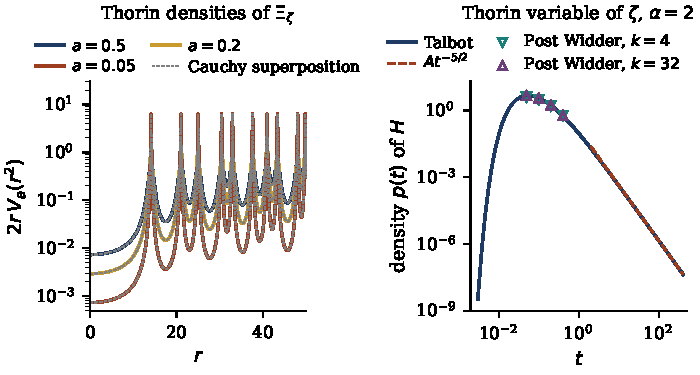
\includegraphics[width=\textwidth]{figs/lap_zeta.pdf}
\caption{Left: Theorem~\ref{thm:lapcauchy} for $\zeta$, the densities $2rV_a(r^2)$ of $\Xi_\zeta$ (Thorin densities for $a\ge\frac12$, and under the Riemann hypothesis below) at basepoints $a=0.5$, $0.2$, $0.05$ (those of $\xi$ at $\frac12+a$), with the Cauchy superpositions over the zeros drawn on top in grey dashed lines; the two agree to $10^{-7}$. Right: Theorem~\ref{thm:laptail}, the density of the Thorin variable of $\zeta$ at $\alpha=2$ by Talbot inversion, its tail $At^{-5/2}$, and the Post Widder approximations with $k=4$ and $32$, on logarithmic axes.}\label{fig:lapzeta}
\end{figure}

\section{Perron's formula as Bromwich inversion}\label{sec:lapperron}

The oldest passage between the two descriptions is classical, and we record it in the language of this chapter; Chapter~\ref{ch:squarefree} uses the same contour shift in \eqref{eq:sf:perron}, for the squarefree ideals of a number field. The undamped Galois face of $\zeta$ is the measure $\nu_0=\sum_n\Lambda(n)\delta_{\log n}$, whose distribution function is Chebyshev's $\psi(e^u)=\sum_{n\le e^u}\Lambda(n)$, and $-\zeta'/\zeta(s)=\int e^{-su}\,d\psi(e^u)$ is its Laplace Stieltjes transform. Bromwich inversion on a line $\operatorname{Re}s=c>1$, taken as a symmetric principal value since $x^s/s$ is not integrable on the line, is Perron's formula \cite{perron1908},
\[
\psi(x)=\frac1{2\pi i}\int_{c-i\infty}^{c+i\infty}\Bigl(-\frac{\zeta'}\zeta(s)\Bigr)\frac{x^s}s\,ds,\qquad x>1\text{ not a prime power},
\]
in which only Galois data enter. Moving the contour to the left across the critical strip, the integrand meets the pole at $s=1$, the zeros $\rho$, the pole at $s=0$, which gives $-\log2\pi$, and the trivial zeros, which give $-\frac12\log(1-x^{-2})$, and the residues give the explicit formula (\cite{davenport2000}, Chapter~17), the sum over $\rho$ being the limit of the sums over $|\gamma|<T$ as $T\to\infty$:
\[
\psi(x)=x-\sum_\rho\frac{x^\rho}\rho-\log2\pi-\tfrac12\log(1-x^{-2}).
\]
The contour shift is the passage: on $\operatorname{Re}s>1$ the integrand is an Euler product, and to the left of the critical strip it is controlled by the functional equation, which for $\zeta$ is the modularity of the theta function. The Cauchy semigroup of Section~\ref{sec:lapcauchy} reaches the zeros by moving a basepoint instead of a contour, with positive measures wherever Theorem~\ref{thm:10dshift}(i) applies. The explicit formula is also used in Section~\ref{sec:05bias} and Chapter~\ref{ch:recip}.

\section{Splines, P\'olya frequency functions and roughness penalties}\label{sec:lapspline}

Two classical papers sit exactly on the arrows of this chapter. Curry and Schoenberg \cite{curryschoenberg1966}, in the full version of their 1947 announcement, developed the fundamental splines, now called B splines, proved that they are probability densities, the volumes of the sections of a simplex, and studied their limits, which are Schoenberg's P\'olya frequency functions \cite{schoenberg1951}, totally positive of every order. Good and Gaskins \cite{goodgaskins1971} estimated a probability density $f$ by maximising the log likelihood minus a roughness penalty $\mathcal R(f)=\omega_1\int(\sqrt f)'^2+\omega_2\int(\sqrt f)''^2$, whose first term is $\frac{\omega_1}4$ times the Fisher information for location, $\int f'^2/f=4\int(\sqrt f)'^2$; they read $e^{-\mathcal R}$ as a prior \cite{goodgaskins1971,goodgaskins1980}, and their second paper used the method to hunt for bumps. De Montricher, Tapia and Thompson \cite{demontrichertapiathompson1975} showed (Proposition~3.5) that with the first penalty alone the estimate is an exponential spline with knots at the observations. So the two papers meet through splines, and both meet the inverse Laplace transforms of this chapter. Inverting a GGC with finitely many Thorin atoms gives a Gamma variable times a B spline variable, Schoenberg's theorem turns GRH into a P\'olya frequency statement (Chapter~\ref{ch:10d}), and among densities vanishing on the walls the Good and Gaskins penalty singles out the Sato Tate law.

\subsection{Atomic Thorin laws invert to B splines}

For $k\ge1$ and knots $u_0\le\dots\le u_k$ with $u_0<u_k$ the Curry Schoenberg B spline is $M(x;u_0,\dots,u_k)=k\,[u_0,\dots,u_k](\cdot-x)_+^{k-1}$, the divided difference in the first variable, read as a confluent one at repeated knots. It is a probability density on $[u_0,u_k]$, and it is the density of $\sum_iu_iP_i$ with $(P_0,\dots,P_k)$ uniform on the simplex, that is Dirichlet with all parameters $1$: the spline is the shadow of a simplex \cite{curryschoenberg1966}. Both facts follow from the classical Hermite Genocchi formula $[u_0,\dots,u_k]\phi=\frac1{k!}\E\phi^{(k)}(\sum_iu_iP_i)$ \cite{deboor2005}.

\begin{theorem}[atomic Thorin laws are Gamma times B spline; after \cite{curryschoenberg1966,jamesroynetteyor2008}]\label{thm:lapspline}
Let $k\ge1$, $0<c_0\le\dots\le c_k$ with $c_0<c_k$, and $H=\sum_iE_i/c_i$ with independent standard exponentials $E_i$, the GGC with Thorin measure $\sum_i\delta_{c_i}$.
\begin{enumerate}
\item[(a)] $H$ has the law of $Y_{k+1}D$, with $Y_{k+1}$ Gamma of shape $k+1$ independent of $D$, whose density is the B spline with knots $1/c_0,\dots,1/c_k$.
\item[(b)] The inverse Laplace transform of $\prod_i(1+s/c_i)^{-1}$ is
\begin{align*}
p_H(t)&=\Bigl(\prod_ic_i\Bigr)(-1)^k[c_0,\dots,c_k]e^{-t\,\cdot}\\
&=\Bigl(\prod_ic_i\Bigr)\frac{t^k}{k!}\int_{c_0}^{c_k}e^{-tx}M(x;c_0,\dots,c_k)\,dx,
\end{align*}
that is $(\prod_ic_i)t^k/k!$ times the Laplace transform of the B spline with knots $c_0,\dots,c_k$. Repeated atoms give repeated knots, with the divided difference read as a confluent one.
\end{enumerate}
\end{theorem}

\begin{proof}
(a) With $Y_{k+1}=\sum_iE_i$ and $P_i=E_i/Y_{k+1}$, $Y_{k+1}$ is Gamma of shape $k+1$, $(P_0,\dots,P_k)$ is Dirichlet with all parameters $1$, and the two are independent by the beta gamma algebra (\cite{jamesroynetteyor2008}, Section~1.4). Then $H=Y_{k+1}D$ with $D=\sum_iP_i/c_i$, which has the B spline density with knots $1/c_i$. (b) For distinct atoms, partial fractions give $p_H(t)=(\prod_jc_j)\sum_ie^{-c_it}/\prod_{j\ne i}(c_j-c_i)$, which is the divided difference written; repeated atoms follow by continuity in the $c_i$. Hermite Genocchi with $\phi(x)=e^{-tx}$, $\phi^{(k)}=(-t)^ke^{-tx}$, gives the second form.
\end{proof}

Part~(a) is the atomic case of the factorisation of James, Roynette and Yor \cite{jamesroynetteyor2008} (Section~1.4, equation~(33)): a GGC whose Thorin measure has finite mass $m$ is a Gamma variable of shape $m$ times an independent Dirichlet mean, by the beta gamma algebra. In part~(b) the first form is the classical density of a sum of independent exponentials, written as a divided difference, and the second is its Peano kernel form \cite{deboor2005}. So inverting the Laplace transform of an atomic Thorin law is a divided difference, and a divided difference is an expectation over a simplex. When the Thorin measure is the image under $1/Q$ of a probability measure $\mu$ restricted to $\{Q>0\}$, as for the Frobenius functionals of Chapter~\ref{ch:recip}, the factorisation can also be written with a standard exponential variable and the Dirichlet mean $\int Q\,dP$ of a Dirichlet process $P$ with base measure $\mu$, and Chapter~\ref{ch:pd} identifies $P$ with the limit of the normalised labelled factorisation of a random integer (Theorem~\ref{thm:pddirichlet}).

For the Hecke GGC $H_N(\ell)$ of Definition~\ref{def:flthecke}, whose $g$ atoms $\ell+1-a_\ell(f)$ have product $|J_0(N)(\mathbb F_\ell)|$ (Chapter~\ref{ch:flt}), part~(b) gives
\[
p_{H_N(\ell)}(t)=|J_0(N)(\mathbb F_\ell)|\,\frac{t^{g-1}}{(g-1)!}\int e^{-tx}M\bigl(x;\{\ell+1-a_\ell(f)\}_f\bigr)\,dx :
\]
the density of the Hecke variable is $t^{g-1}$ times the Laplace transform of a B spline whose knots are the atoms. The atom of a rational $f$, attached to an elliptic curve $E_f$, is the point count $|E_f(\mathbb F_\ell)|$, but only the product of all the atoms is always a point count. Hecke atoms can repeat, for example at $(N,\ell)=(37,7)$ and $(113,2)$, and then the knots repeat; at $(37,7)$ both atoms are $9$, the B spline degenerates to the point mass at $9$, and $H_{37}(7)$ is a Gamma variable of shape $2$ and rate $9$. For $N=67$, $\ell=2$, the five atoms are $1$, $2.382$, $3.382$, $4.618$, $5.618$ with product $209=|J_0(67)(\mathbb F_2)|$. Computed exactly, the B spline formula agrees with the partial fraction density to within $6\cdot10^{-15}$ on $[0,4]$, and a histogram of $400000$ samples of $Y_5D$ agrees with both within sampling error (Figure~\ref{fig:lapspline}, right).

\subsection{P\'olya frequency functions and GRH}

Schoenberg's theorem (Theorem~\ref{thm:ch10schoenberg}) characterises the P\'olya frequency functions, totally positive of every order, by their bilateral Laplace transforms, the reciprocals of functions of the Laguerre P\'olya class, and Curry and Schoenberg showed that these functions arise as limits of their B splines \cite{curryschoenberg1966}. Through Schoenberg's theorem, Theorem~\ref{thm:10dvdp} and the remark after its proof show that GRH for $\pi$ holds if and only if $t\mapsto\Xi_\pi(0)/\Xi_\pi(t)$ is the characteristic function of a symmetric P\'olya frequency density, that of $V_\pi=\sum_kL_k/\gamma_k$, with independent standard Laplace variables $L_k$, which has the law of $\sqrt{2Z_\pi}\,N$, where $Z_\pi$ is the explosion time of Theorem~\ref{thm:hitexplosion} and $N$ is standard normal and independent of $Z_\pi$ (for $\xi$, \cite{roynetteyor2005,polson2018vdp,konstantopoulospatiesarkar2024}). Under GRH the density of $V_\pi$ is therefore a limit of B spline densities, and its truncation to the first $K$ zeros is a difference $\sum_{k\le K}E_k/\gamma_k-\sum_{k\le K}E'_k/\gamma_k$ of two independent hypoexponential variables, each a Gamma variable times a B spline variable by Theorem~\ref{thm:lapspline}. The bilateral Laplace transform of $V_\pi$ is $\E e^{sV_\pi}=\E e^{s^2Z_\pi}$, the transform of the explosion time continued to negative argument.

\subsection{The Sato Tate law minimises the Good and Gaskins penalty}

Let $G$ be a compact connected simply connected Lie group, such as $\SU(2)$ or $\USp(2n)$, with alcove $\mathcal A$, positive roots $\alpha$ and half sum $\rho_G$, and give the Lie algebra of a maximal torus the invariant inner product in which, for $\SU(2)$ and $\USp(2n)$, the eigenvalue angles are orthonormal coordinates. By Weyl's integration formula (Theorem~\ref{thm:ch6weyl}) the image of Haar measure on conjugacy classes, the Sato Tate law of Chapter~\ref{ch:04} for $\SU(2)$ and of Chapter~\ref{ch:12} for $\USp(4)$, has density $f_G=c|\Delta_G|^2$ on $\mathcal A$, with $\Delta_G=\prod_{\alpha>0}(e^{i\alpha/2}-e^{-i\alpha/2})$. By the Weyl character formula $\Delta_G\chi_\lambda=\sum_w\operatorname{sgn}(w)e^{iw(\lambda+\rho_G)}$, an eigenfunction of the Laplacian with eigenvalue $|\lambda+\rho_G|^2$ that vanishes on the walls of $\mathcal A$; for $\lambda=0$ it has constant sign inside $\mathcal A$.

\begin{theorem}[Sato Tate is the Good and Gaskins ground state; this book, after \cite{huber1974,berard1980}]\label{thm:lapgg}
Among densities $f$ on $\mathcal A$ such that $\sqrt f$ vanishes on the boundary $\partial\mathcal A$ and $\int_{\mathcal A}|\nabla\sqrt f|^2<\infty$, the Good and Gaskins roughness $\int_{\mathcal A}|\nabla\sqrt f|^2$, one quarter of the trace of the Fisher information for location, is at least $|\rho_G|^2$, with equality exactly for the Sato Tate law $f_G$. For $G=\SU(2)$, with $\theta\in[0,\pi]$ and $\sqrt f=\sqrt{2/\pi}\sum_jb_j\sin j\theta$, $\sum_jb_j^2=1$,
\[
\int_0^\pi\bigl((\sqrt f)'\bigr)^2d\theta=\sum_jj^2b_j^2,\qquad \frac{\sin j\theta}{\sin\theta}=\tr\Sym^{j-1}\begin{pmatrix}e^{i\theta}&0\\0&e^{-i\theta}\end{pmatrix},
\]
so the roughness is the Laplace eigenvalue energy $\sum_\lambda|\lambda+\rho_G|^2b_\lambda^2$, which is $|\rho_G|^2$ plus the Casimir energy, in the basis of symmetric power characters, and the Sato Tate law is $b=e_1$. Given angles $\theta_1,\dots,\theta_n$, put $\hat m_j=\frac1n\sum_{i=1}^n\tr\Sym^{j-1}(\theta_i)$, the trace being that of the matrix above. Near the Sato Tate law, the maximiser of $\frac1n\sum_i\log f(\theta_i)-\omega\int_0^\pi(\sqrt f)'^2$ over $\sqrt f=\sqrt{2/\pi}\sum_{j\le J}b_j\sin j\theta$ satisfies
\[
b_j=\frac{\hat m_j}{2+\omega(j^2-1)}+O\Bigl(\max_{2\le l\le2J-1}\hat m_l^2\Bigr),\qquad 2\le j\le J .
\]
\end{theorem}

\begin{proof}
The functions $\Delta_G\chi_\lambda$ restricted to $\mathcal A$, with $\lambda$ dominant, are a complete orthogonal system of Dirichlet eigenfunctions of the Laplacian on $\mathcal A$, by the Weyl character formula and the Peter Weyl theorem (Theorem~\ref{thm:A:pw}), with eigenvalues $|\lambda+\rho_G|^2$; the smallest is $|\rho_G|^2$, at $\lambda=0$, and it is simple. The Rayleigh quotient of $\sqrt f$, with $\int f=1$, is $\int|\nabla\sqrt f|^2\ge|\rho_G|^2$, with equality only for $\sqrt f=c|\Delta_G|$, which is $f=f_G$. For $\SU(2)$, $\mathcal A=[0,\pi]$, $\rho_G=1$, $\Delta_G\chi_{j-1}=2i\sin j\theta$, and $\int(\sum_jb_j\sqrt{2/\pi}\sin j\theta)'^2=\sum_jj^2b_j^2$. For the maximiser write $b=(\sqrt{1-|\epsilon|^2},\epsilon_2,\dots,\epsilon_J)$ and $\sin j\theta/\sin\theta=U_{j-1}(\cos\theta)$. Then $\frac1n\sum_i\log f(\theta_i)$ is a constant plus $2\sum_j\epsilon_j\hat m_j-|\epsilon|^2-\sum_{j,k}Q_{jk}\epsilon_j\epsilon_k+O(|\epsilon|^3)$, where $Q_{jk}=\frac1n\sum_iU_{j-1}(\cos\theta_i)U_{k-1}(\cos\theta_i)$ is the sum of the $\hat m_l$ over $l=|j-k|+1,|j-k|+3,\dots,j+k-1$ by the Clebsch Gordan rule, with $\hat m_1=1$, so that $Q_{jk}=\delta_{jk}+O(\max_l|\hat m_l|)$. The penalty is $\omega(1+\sum_j(j^2-1)\epsilon_j^2)$. At the stationary point $(2+\omega(j^2-1))\epsilon_j=\hat m_j+O(|\epsilon|\max_l|\hat m_l|+|\epsilon|^2)$, and $\epsilon=O(\max_l|\hat m_l|)$ gives the formula: the cross terms $\epsilon_j\epsilon_k$ have coefficients $O(\max_l|\hat m_l|)$, so they change $b$ only at second order.
\end{proof}

For $\SU(2)$ the inequality is Huber's theorem that among laws on an interval the sine squared arch has least Fisher information \cite{huber1974}; in general it is the Rayleigh principle for the Dirichlet Laplacian of the alcove, whose spectrum B\'erard computed \cite{berard1980} (Proposition~9).

For $\USp(4)$, with $\sqrt f\propto(\cos\theta_1-\cos\theta_2)\sin\theta_1\sin\theta_2=\frac12(\sin2\theta_1\sin\theta_2-\sin\theta_1\sin2\theta_2)$ on $0<\theta_2<\theta_1<\pi$, the eigenvalue is $5=|\rho_G|^2$, $\rho_G=(2,1)$, and the normalising constant is $16/\pi^2$, twice the constant of Proposition~\ref{thm:12usp4}, which integrates over the square $[0,\pi]^2$. In the Bayesian reading of Good and Gaskins, with the prior $e^{-n\omega\int(\sqrt f)'^2}$ for $n$ angles, the Sato Tate law is, formally, the mode of the prior among densities whose square root vanishes on the walls, and the posterior mode is the maximiser of the theorem. Since the fitted value of $\hat m_j$, the mean of $\tr\Sym^{j-1}$, is about $2b_j$, the posterior mode shrinks the empirical moment $\hat m_j$ by the factor $(1+\omega(j^2-1)/2)^{-1}$: the larger the representation, the stronger the shrinkage. The $\hat m_j$ are the Weyl averages $W_\rho(n)$, $\rho=\Sym^{j-1}$, of Chapter~\ref{ch:12}, and the roughness prior is a nonparametric alternative of the kind discussed there, where the Bayesian identification compares finitely many candidate groups.

Figure~\ref{fig:lapspline} fits the Good and Gaskins estimate with twelve sine terms to the Frobenius angles of two curves. For $11a1$, with the $664578$ primes below $10^7$ other than $11$, the moments $\hat m_2,\dots,\hat m_7$ are of size $4\cdot10^{-4}$, the estimate is indistinguishable from the Sato Tate law (roughness $1.0001$ at $\omega=0.01$), and the exact maximiser agrees with the first order formula to within $0.7$ percent for $j\le6$ and $\omega=0.01,0.1,1$. For the curve $E_2\colon y^2=x^3-x$ of Chapter~\ref{ch:01} (conductor $32$, complex multiplication by $\Z[i]$), with the $78497$ odd primes below $10^6$, the angle law is $\mu_{\mathrm{CM}}$, $\frac12\delta_{\pi/2}$ plus half the uniform law, so $\E\tr\Sym^{2m}=\frac12((-1)^m+1)$ (Proposition~\ref{prop:04cm}). The data give $\hat m_3=-0.0033$ and $\hat m_5=0.998$, against $0$ and $1$, and the estimate at $\omega=0.01$ has $b_5=0.334$ and a spike at $\pi/2$; at $\omega=1$ the prior pulls it back to $b_5=0.035$, close to the Sato Tate shape. Here the first order formula is only qualitative, because this curve is far from Sato Tate.

\begin{figure}[!htbp]
\centering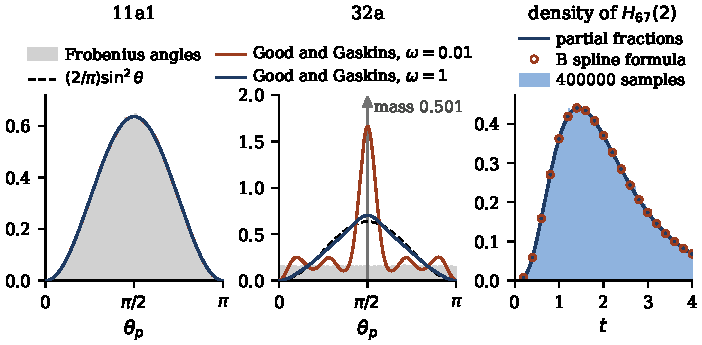
\includegraphics[width=\textwidth]{figs/lap_spline.pdf}
\caption{Left and centre: Theorem~\ref{thm:lapgg}. Good and Gaskins estimates of the Frobenius angle density with $\omega=0.01$ and $\omega=1$, against the Sato Tate law $\frac2\pi\sin^2\theta$ and over histograms of the angles, for $11a1$ (primes below $10^7$ other than $11$) and for $E_2$, of class $32a$ (odd primes below $10^6$). The atom of $E_2$ at $\pi/2$, from the primes with $a_p=0$, is drawn as an arrow labelled with its mass, and the bars show the other angles; the estimate with $\omega=0.01$ has a spike there. Right: Theorem~\ref{thm:lapspline}. The density of the Hecke GGC $H_{67}(2)$ by partial fractions and by the B spline formula computed exactly, over a histogram of $400000$ samples of a Gamma variable times a B spline variable.}\label{fig:lapspline}
\end{figure}

\subsection{Open problems}

\begin{problem}[Stable recovery of Frobenius from a window]\label{op:lapwindow}
By Theorem~\ref{thm:lapfaces}(iii) the transported density $g_\alpha$ on any interval $[0,r_0)$ determines every $\Lambda_L(n)$, but only through analytic continuation, which is unstable. Suppose $g_\alpha$ is known on $[0,r_1]$ to within $\eta$. Corollary~\ref{cor:lapfrob}, with the Gaussian mean truncated at $r_1$, recovers $\Lambda_L(n)$ to within $\varepsilon$ once $\eta$ is of order $\varepsilon n^{-\alpha}$ and $r_1$ of order $n\log(n^\alpha/\varepsilon)$. Is an interval of length of order $n$, the reciprocal of the gap $\log(1+1/n)$ between the frequencies $\log n$ and $\log(n+1)$, necessary for every stable method, as Ingham's inequality for nonharmonic Fourier series \cite{ingham1936} suggests? A positive answer would be an uncertainty principle for the Galois face, comparable with the bounds in effective Chebotarev theorems \cite{lagariasodlyzko1977}.
\end{problem}

\begin{problem}[Good and Gaskins for Thorin densities]\label{op:lapgg}
The inversions of this chapter are exact but need exact input. Treat the ordinates $0<\gamma_1\le\dots\le\gamma_K$ as a sample from the normalised counting measure of the zeros, or the transported density on a grid as noisy data; define the penalised likelihood of Good and Gaskins for the square root of the Thorin density $U_{\mathrm{ar}}$ of Section~\ref{sec:10daway}, or for the density of $H$; identify its maximiser as de Montricher, Tapia and Thompson did; and compare its error with that of the Gaussian means of Theorem~\ref{thm:lapbohr} on the same input.
\end{problem}

\section{Notes}

Lerch's theorem (Chapter~II, Theorems~6.2 and 6.3), the complex inversion formula (Chapter~II, Theorem~7.3, and Chapter~VI, Theorem~5a) and the real inversion formula, found by Post and extended by Widder (Chapter~VII), are in Widder's book \cite{widder1941}; Feller \cite{feller1971} reads the last as a law of large numbers. Talbot's contour \cite{talbot1979} and the framework of Abate and Whitt \cite{abatewhitt2006} are the standard numerical inversions, and Stieltjes inversion is classical \cite{stieltjes1894,akhiezer1965}. Theorem~\ref{thm:lapbohr} and Corollary~\ref{cor:lapfrob} are Bohr's formula for the Fourier coefficients of an almost periodic function and its uniqueness theorem, for Dirichlet series in Besicovitch \cite{besicovitch1932} (Chapter~I, Sections~3 and 4; Chapter~III, Section~3), and Theorem~\ref{thm:lapfaces} combines them with the uniqueness of Dirichlet series. Proposition~\ref{prop:lappolya} is Hecke's Mellin integral (\cite{hecke1936}, Section~2), which goes from the $L$ function to the form, the reverse of Section~\ref{sec:02mellin} and \eqref{eq:recipmellin}; that the inverse transform is modular for all of $\Gamma_0(N)$ is Weil's converse theorem \cite{weil1967} (Satz~2), and for two dimensional Artin representations it is Th\'eor\`eme~4.10 of Deligne and Serre \cite{deligneserre1974}. Perron's formula is \cite{perron1908}, and the explicit formula for $\psi$ is in \cite{davenport2000}.

The $2\sin^2$ lemma is Lemma~14 of \cite{polson2018vdp} (see also \cite{polson2017}, Section~5), with its first step from Roynette and Yor \cite{roynetteyor2005}, Th\'eor\`eme~I.1.1, as recorded in Chapter~\ref{ch:10d}, where its Thorin consequences are developed. The Poisson kernel form of Theorem~\ref{thm:lapcauchy} is in the proof of Theorem~\ref{thm:10dshift}, in Proposition~\ref{prop:10dsmooth} and in \cite{polson2018vdp} (Theorem~18 and Remark~21), and the backward Cauchy flow is in \cite{polson2017} (Section~8 and Theorem~9.2), whose Theorem~8.2 writes, for $\xi$, the distribution function of the measure of Theorem~\ref{thm:lapcauchy} as a sum of arctangents; Theorem~\ref{thm:lapcauchy} restates it through folded Cauchy variables and for every self dual $\pi$. The criterion of Hinkkanen and Lagarias \cite{hinkkanen1997,lagarias1999} adds the same Poisson kernels. The P\'olya frequency form of GRH is Theorem~\ref{thm:10dvdp}, for $\xi$ in \cite{roynetteyor2005} (Th\'eor\`eme~V.3.2), \cite{polson2018vdp} and \cite{konstantopoulospatiesarkar2024}. Theorem~\ref{thm:laptail} is due to Roynette and Yor \cite{roynetteyor2005}, whose proof is Tauberian; ours uses Doetsch's transfer theorem for Laplace transforms with algebraic singularities \cite{doetsch1974}.

The B splines and their limits are from Curry and Schoenberg \cite{curryschoenberg1966}, the Peano kernel and Hermite Genocchi forms of a divided difference are in de Boor's survey \cite{deboor2005}, P\'olya frequency functions are from Schoenberg \cite{schoenberg1951} and Karlin \cite{karlin1968}, and the Gamma times Dirichlet mean structure of GGCs, whose atomic case is Theorem~\ref{thm:lapspline}(a), is from James, Roynette and Yor \cite{jamesroynetteyor2008} (Section~1.4). The roughness penalty and its Bayesian reading are from Good and Gaskins \cite{goodgaskins1971,goodgaskins1980}, its exponential spline solutions from de Montricher, Tapia and Thompson \cite{demontrichertapiathompson1975}; Good's earlier work on Poisson summation \cite{good1962} appears in Chapter~\ref{ch:recip}. The inequality of Theorem~\ref{thm:lapgg} is Huber's for $\SU(2)$ \cite{huber1974} and the Rayleigh principle for the alcove in general \cite{berard1980}, the ground state being the Weyl denominator. New here as formulated, as far as we know, are the Gaussian error bounds of Theorem~\ref{thm:lapbohr} and Corollary~\ref{cor:lapfrob}, the Hecke reading of Theorem~\ref{thm:lapspline}, the Good and Gaskins reading of the Sato Tate law in Theorem~\ref{thm:lapgg}, with its expansion in symmetric power characters and its shrinkage formula, and the computations.

\section{Exercises}

\begin{enumerate}
\item Apply Theorem~\ref{thm:lappostwidder} to $g(x)=e^{-x}$ and show that the $k$th Post Widder approximation is $(1+t/k)^{-k-1}$.
\item Use the weak form of Theorem~\ref{thm:lapstieltjes}, integrating $\frac1\pi\operatorname{Im}(\varphi'/\varphi)(-z+i\epsilon)$ against test functions, to show that the Gamma law with shape $m$, $\varphi(s)=(1+s)^{-m}$, has Thorin measure $m\delta_1$.
\item Derive the identity of Theorem~\ref{thm:lapbohr} for a single atom $\nu=c\delta_x$, and, for $\nu=\delta_1+\delta_{1.01}$, find the smallest window $R$ for which the Gaussian mean $\mathcal G_R$ recovers the weight at $x=1$ to $10^{-6}$.
\item Show that the quadruple $z,-z,\bar z,-\bar z$ of zeros of $\Xi^{\mathrm{sd}}_\pi$, $z=\beta+i\gamma$, $0<\beta<a$, contributes $\operatorname{Law}(|\gamma+(a-\beta)C|)+\operatorname{Law}(|\gamma+(a+\beta)C|)$ to the Thorin measure of Theorem~\ref{thm:lapcauchy}, of total mass $2$, the same as two zeros of $L(s,\pi)$ on the critical line in the upper half plane.
\item For the Dedekind zeta function of $\Q(i)$, compute numerically $A$ of Theorem~\ref{thm:laptail} at $\alpha=2$ and compare it with the constant for $\zeta$.
\item Show that the B spline with two knots $u_0<u_1$ is the uniform density on $[u_0,u_1]$, and deduce from Theorem~\ref{thm:lapspline} the density of $E_0/c_0+E_1/c_1$.
\item Show that the Fisher information for location of the Sato Tate angle law $\frac2\pi\sin^2\theta$ on $[0,\pi]$ is $4$, and that no density on $[0,\pi]$ vanishing at the ends has smaller Fisher information.
\item Check Perron's formula numerically for $x=100.5$ by integrating along $\operatorname{Re}s=2$, $|\operatorname{Im}s|\le T$, and observe the convergence in $T$.
\end{enumerate}

\section{Open computational problems}

The scripts named below are in \texttt{laplace/code/} (Section~\ref{sec:B:scripts}).

\begin{compproblem}[Four faces of elliptic curves]\label{cp:lapfaces}
Objective: carry out the inversions of this chapter for elliptic curves of both root numbers. Recover $\Lambda_E(n)$ for $n\le100$ from the transported density $g_\alpha$ by the Gaussian means of Corollary~\ref{cor:lapfrob}, with the smallest window that gives each value to $10^{-6}$; rebuild the P\'olya kernel $\Phi_E$ of Proposition~\ref{prop:fltsymmetric} from $\Lambda(1+it,E)$ by Bromwich inversion and compare it with the kernel summed from the $q$ expansion; and compare the densities $V_a$ of $\Xi^{\mathrm{sd}}_E$ at $a=0.5$, $0.2$ and $0.05$ with the Cauchy superpositions of Theorem~\ref{thm:lapcauchy} over the zeros. Objects and scale: $11a1$ and $37a1$, as Figure~\ref{fig:lapfaces} does for the weight one form, then one curve from each isogeny class of conductor below $100$; Dirichlet coefficients to $10^5$; basepoints $\alpha\in\{1.5,2\}$ for $L(s+\frac12,E)$, whose coefficients are $\Lambda_E(n)n^{-1/2}$; windows up to $10^3$; zeros to height $100$. Route: \texttt{switch23.py} and \texttt{switch23b.py}, with the eta quotient replaced by the $L$ function of the curve (PARI/GP \texttt{lfuncreate}, \texttt{lfunlambda} on the critical line, \texttt{lfunzeros}); Gaussian means by quadrature truncated at six windows, as in Section~\ref{sec:lapbohr}, with the bound of Corollary~\ref{cor:lapfrob} for a finite window and a separate bound for the truncation. Deliverable: tables of the recovered $\Lambda_E(n)$, their errors and the minimal windows against $n$, with a fitted law for the window, the numerical side of Open Problem~\ref{op:lapwindow}; the maximal difference of the two kernels on $|u|\le3$, the kernel of $37a1$ being odd; and the residuals of the Cauchy superpositions. Why it matters: the Frobenius traces of the weight one form take three values at the unramified primes, while for an elliptic curve they follow the Sato Tate law and the kernels have both parities, so the problem tests the inverse arrows on the forms that carry the modularity of Chapter~\ref{ch:flt}, and it measures how pessimistic the bound of Corollary~\ref{cor:lapfrob} is.
\end{compproblem}

\begin{compproblem}[Zeros from the heat trace by Post Widder]\label{cp:lappw}
Objective: invert the heat trace by the Post Widder formula. With $N(t)$ the number of ordinates $\gamma>0$ with $\gamma^2\le t$, $\mathcal W(x)/x=\int_0^\infty e^{-xt}N(t)\,dt$, and the identity of Theorem~\ref{thm:lappostwidder}, which holds for $g$ of polynomial growth such as $N$, writes the $k$th approximation as a Gamma smoothing of $N$ of relative width about $k^{-1/2}$; find the order $k$ and the working precision at which the step of $N$ at the $j$th zero is resolved. Objects and scale: $L(s,\Delta)$, $\zeta$ and $L(s,\rho)$ for the $S_3$ representation of $x^3-x-1$; the first $50$ ordinates; orders $k\le10^3$. Route: $\mathcal W$ and its derivatives from the primes through the explicit formula \eqref{eq:10dweil}, or from Frobenius traces through Definition~\ref{def:recipheat}, in ball arithmetic, the pipeline of the derivative tests of Problem~\ref{cp:recipicosa}; the sums over the zeros as a check. Deliverable: for each function and each $j\le50$ the smallest $k$ and the precision that resolve the $j$th step, compared, at equal cost, with the Gaussian bump of Figure~\ref{fig:10dprimes} and the Cauchy smoothing of Theorem~\ref{thm:lapcauchy}. Why it matters: the derivatives $(-1)^k\mathcal W^{(k)}$ are the quantities whose signs the complete monotonicity criteria of Theorems~\ref{thm:10bmain} and \ref{thm:recipcm} concern; the problem measures how much of the zero set a given number of them determines, and whether the slow convergence of Post Widder, an error of order $1/k$, can be paid for by the accuracy of the explicit formula at small $x$.
\end{compproblem}

\begin{compproblem}[Thorin laws in the strip by Talbot inversion]\label{cp:laptalbot}
Objective: for a completed $L$ function $f$ and basepoints $\alpha$ inside and to the right of the critical strip, invert by Talbot's contour the transform $\varphi_\alpha(s)=e^{b\sqrt s}f(\alpha)/f(\alpha+\sqrt s)$, $b=(f'/f)(\alpha)$, whose Thorin density is the density $U$ of \eqref{eq:10dU}; record where the inverted density is negative, and compare its mean and its tail with $\frac12(\log f)''(\alpha)$ and with the constant $-(\log f)'''(\alpha)/(8\sqrt\pi)$ of the proof of Theorem~\ref{thm:laptail}. Objects and scale: $\xi$, $\Lambda(s,\Delta)$ at the same offsets $\alpha-\frac12$ from its centre, and $\Lambda(s,\chi_{-4})$; the basepoints $0.55$, $0.75$, $0.99$, $1.25$ and $2$ of Section~\ref{sec:10daway}; $5\cdot10^{-4}\le t\le10^4$. Route: \texttt{zeta\_tail.py}, which does this for $\zeta$ at $\alpha=2$, with $\zeta$ replaced by the completed function, $f$ and $f'/f$ from mpmath or PARI/GP \texttt{lfunlambda} at $30$ digits; Talbot's contour checked against the Euler algorithm of Abate and Whitt \cite{abatewhitt2006}; error bounds from the size of $\varphi_\alpha$ on the contour. Deliverable: the densities with their minima, total masses and means, fitted tail constants with standard errors against the predicted ones, and for each function the smallest basepoint at which the computed density is positive on the grid. Why it matters: Theorem~\ref{thm:laptail} needs nonnegative Dirichlet coefficients; for a completed function $\varphi_\alpha$ is a GGC transform exactly where $U\ge0$, which for $\xi$ holds under the Riemann hypothesis, is known for $\alpha\ge1$ and is open below (Section~\ref{sec:10daway}, Open Problem~\ref{op:recipdescent}); the inverted laws are the probabilistic content of that positivity, and a density positive on a grid verifies nothing about the zeros.
\end{compproblem}
